\documentclass[11pt]{article}
\usepackage[margin=1in]{geometry}
\usepackage{amsmath,amssymb,bm}
\usepackage{graphicx}
\usepackage{booktabs}
\usepackage{subcaption}
\usepackage{enumitem}
\usepackage{xcolor}
\usepackage[colorlinks=true,linkcolor=blue,urlcolor=blue]{hyperref}

\graphicspath{{../codes/figs/}}

\newcommand{\piold}{\pi_{\theta_{\mathrm{old}}}}
\newcommand{\Ahat}{\hat{A}}
\newcommand{\E}{\mathbb{E}}
\newcommand{\Ehat}{\hat{\mathbb{E}}}
\newcommand{\code}[1]{\texttt{#1}}

\title{ECE 562 Assignment 3: PPO II\\[2pt]}
\author{Emmanuel Oluwasegun Olateju (\href{mailto:eolateju@ualberta.ca}{eolateju@ualberta.ca})}
\date{\today}

\begin{document}
\maketitle

\section*{Section 1: Theory}
\textbf{Notation and assumptions} (as given in the assignment):
\begin{itemize}
  \item Support assumptions:
        $\pi_\theta(a|s) > 0 \;\Rightarrow\; \piold(a|s) > 0$, \quad
        $d^{\pi_\theta}(s) > 0 \;\Rightarrow\; d^{\piold}(s) > 0$.

  \item $p_0$: initial state distribution; \quad
        $P(s'|s,a)$: transition kernel (fixed by the environment, does not depend on the policy).

  \item \textbf{Normalized State-visitation distribution of a policy:}
        \[
          d^{\pi}(s) \;=\; (1-\gamma)\sum_{t=0}^{\infty} \gamma^t \, P(s_t = s \mid s_0 \sim p_0, \pi)
        \]

  \item \textbf{Policy Gradient Theorem (With Normalization):}
        \[
          \nabla_\theta J(\theta) \;=\; \frac{1}{1-\gamma}\,
          \E_{s \sim d^{\pi_\theta},\, a \sim \pi_{\theta}}
          \!\left[\nabla_\theta \log \pi_\theta(a|s)\, A^{\pi_\theta}(s,a)\right]
        \]

  \item \textbf{Per-step importance ratio:}
        \[
          r_\theta(s,a) \;=\; \frac{\pi_\theta(a|s)}{\piold(a|s)}
        \]
\end{itemize}


\subsection*{Q1}
\begin{itemize}
  \item Trajectories of fixed length $T$:
        \[
          \tau = (s_0, a_0,\; s_1, a_1, \ldots, s_{T-1},\, a_{T-1},\, s_T)
        \]
  \item The reward $r_t$ depends only on $(s_t, a_t, s_{t+1})$, and the discounted return is
        \[
          R(\tau) \;=\; \sum_{t=0}^{T-1} \gamma^t r_t
        \]

  \item \textbf{Finite-horizon objective:}
        \[
          J_T(\theta) \;=\; \E_{\tau \sim \pi_\theta}\!\bigl[R(\tau)\bigr]
          \;=\; \sum_\tau p_\theta(\tau)\,R(\tau)
        \]

  \item \textbf{Trajectory probability:}
        \[
          p_\theta(\tau) \;=\; p_0(s_0)\prod_{t=0}^{T-1} \pi_\theta(a_t|s_t)\,P(s_{t+1}|s_t, a_t)
        \]
\end{itemize}

\begin{enumerate}[label=(\alph*)]
  \item Start from the definition and multiply and divide by $p_{\theta_{\text{old}}}(\tau)$:
        \[
          J_T(\theta) \;=\; \sum_\tau p_\theta(\tau)\, R(\tau)
          \;=\; \sum_{\tau:\, p_{\theta_{\text{old}}}(\tau) > 0} p_{\theta_{\text{old}}}(\tau)\,
          \frac{p_\theta(\tau)}{p_{\theta_{\text{old}}}(\tau)}\, R(\tau)
          \;=\; \E_{\tau \sim \piold}\!\left[\frac{p_\theta(\tau)}{p_{\theta_{\text{old}}}(\tau)}\, R(\tau)\right].
        \]

        \textbf{Where the support assumption is used:} dividing by $p_{\theta_{\text{old}}}(\tau)$
        is only allowed when $p_{\theta_{\text{old}}}(\tau) > 0$ which is possible only when
        $p_{\theta}(\tau) > 0$ according to the support assumpion; therfore, the ratio $\frac{p_{\theta}(\tau)}{p_{\theta_{\text{old}}}(\tau)}$ cannot explode ito infinity. So the middle step keeps only those trajectories with  $p_{\theta}(\tau) > 0$. This drops nothing from the original sum: both trajectory probabilities share the same
        $p_0$ and $P$, and $\pi_\theta(a_t|s_t) > 0 \Rightarrow \piold(a_t|s_t) > 0$ at every step, so
        $p_\theta(\tau) > 0 \Rightarrow p_{\theta_{\text{old}}}(\tau) > 0$. Any trajectory with
        $p_{\theta_{\text{old}}}(\tau) = 0$ therefore also has $p_\theta(\tau) = 0$ and contributes zero to
        $J_T(\theta)$. The last step is the definition of an expectation under $p_{\theta_{\text{old}}}$.

  \item
        \[
          \frac{p_\theta(\tau)}{p_{\theta_{\text{old}}}(\tau)}
          \;=\;
          \frac{p_0(s_0)\displaystyle\prod_{t=0}^{T-1}\pi_\theta(a_t|s_t)\,P(s_{t+1}|s_t,a_t)}
          {p_0(s_0)\displaystyle\prod_{t=0}^{T-1}\piold(a_t|s_t)\,P(s_{t+1}|s_t,a_t)}
          \;=\;
          \prod_{t=0}^{T-1}\frac{\pi_\theta(a_t|s_t)}{\piold(a_t|s_t)}
        \]

        Both policies act in the same environment and we evaluate the same trajectory $\tau$, so
        $p_0(s_0)$ and every $P(s_{t+1}|s_t,a_t)$ appear identically in the numerator and the
        denominator and cancel. What is left only needs the probabilities that $\pi_\theta$ and $\piold$
        give to the actions that were actually taken, which we can always compute from the policy networks.

        This matters for model-free RL because we do not know $p_0$ or $P$. If the ratio depended on
        them we would need a model of the environment to reweight old trajectories. Because they cancel,
        trajectories collected by $\piold$ can be reweighted using only the policies.

  \item The trajectory weight is a product of $T$ per-step ratios:
        \[
          \prod_{t=0}^{T-1}\frac{\pi_\theta(a_t|s_t)}{\piold(a_t|s_t)}
          \;=\;
          \prod_{t=0}^{T-1} r_{\theta}(s_t, a_t).
        \]
        Even if each ratio is only slightly different from 1, the differences multiply over time
        (e.g.\ $1.1^{T}$ grows very large and $0.9^{T}$ goes to zero for long $T$). For long horizons the
        weights of most trajectories become almost zero while a few become huge, so the estimate is
        dominated by a handful of trajectories and its variance grows very fast with $T$. This makes
        the gradient estimate too noisy to be useful.

        PPO instead uses the single-step ratio $r_\theta(s_t, a_t)$ for each sample. This has much lower
        variance, but it is an approximation: it ignores how the earlier action changes affect which
        states are reached, i.e.\ it leaves out the state-distribution correction discussed in Q2.
        This is acceptable only when $\pi_\theta$ stays close to $\piold$.
\end{enumerate}


\subsection*{Q2}
\begin{itemize}
  \item Samples come from the behaviour policy: $s \sim d^{\piold}(s)$, \; $a \sim \piold(a|s)$.

  \item Full state-action distribution ratio:
        \[
          \frac{d^{\pi_{\theta}}(s)\;\pi_\theta(a|s)}{d^{\piold}(s)\;\piold(a|s)}
          \;=\; w_\theta(s)\,r_{\theta}(s,a),
          \qquad
          w_\theta(s) \;=\; \frac{d^{\pi_\theta}(s)}{d^{\piold}(s)}
        \]
\end{itemize}

\begin{enumerate}[label=(\alph*)]
  \item Our data has distribution $d^{\piold}(s)\,\piold(a|s)$. Multiplying by $r_\theta(s,a)$ only
        changes the action part:
        \[
          d^{\piold}(s)\,\piold(a|s)\cdot r_\theta(s,a) \;=\; d^{\piold}(s)\,\pi_\theta(a|s).
        \]
        So after reweighting, actions are distributed as under $\pi_\theta$ for each given state, but
        the states are still weighted by how often the \emph{old} policy visited them, $d^{\piold}(s)$.
        Turning $d^{\piold}(s)$ into $d^{\pi_\theta}(s)$ would require the extra factor $w_\theta(s)$,
        which PPO does not use. In other words, $r_\theta$ corrects ``which action is taken in $s$'', but
        not ``how often $s$ is visited''.

        The older the policy that generated the data, the more $\pi_\theta$ has moved away from it.
        Different policies take different actions, which lead to different states, so $d^{\pi_\theta}$
        and $d^{\piold}$ drift further apart and $w_\theta(s)$ moves further from 1. Ignoring
        $w_\theta(s)$ (setting it to 1) therefore causes a larger error: the update gives too much weight
        to states the current policy rarely visits and too little to states it visits often.

  \item
        \begin{itemize}
          \item Total variation distance:
                \[
                  D_{TV}(p, q) \;=\; \frac{1}{2}\sum_{a} \left| p(a) - q(a) \right|
                \]

          \item Known bound (Achiam et al., 2017):
                \[
                  \big\| d^{\pi_\theta} - d^{\piold} \big\|_1
                  \;\le\; \frac{2\gamma}{1-\gamma}\;
                  \E_{s \sim d^{\piold}}\!\Big[ D_{TV}\big(\pi_\theta(\cdot|s),\, \piold(\cdot|s)\big) \Big]
                \]
        \end{itemize}

        The left side is the total state-visitation mismatch. The right side is a constant times the
        average difference between the two action distributions, averaged over states from
        $d^{\piold}$, which are exactly the states in our batch. If $\pi_\theta$ stays close to $\piold$
        in every visited state, $D_{TV}$ is small, so the state-visitation mismatch is also small,
        $d^{\pi_\theta} \approx d^{\piold}$, and $w_\theta(s) \approx 1$. In that case dropping
        $w_\theta(s)$ only causes a small error.

        PPO's clipped objective
        \[
          \min\!\big(r_\theta(s,a)\,\Ahat(s,a),\;
          \mathrm{clip}(r_\theta(s,a), 1-\epsilon, 1+\epsilon)\,\Ahat(s,a)\big)
        \]
        helps keep the update small: once a sample's ratio has moved past $1+\epsilon$ (for
        $\Ahat > 0$) or below $1-\epsilon$ (for $\Ahat < 0$), the clipped term is selected and that sample
        gives zero gradient. So there is no incentive to push $\pi_\theta$ further away from $\piold$ on
        that sample, which indirectly keeps $D_{TV}$, and therefore the state mismatch, small.

        \textbf{Does clipping strictly enforce a bound on $D_{TV}$? No.} Clipping only removes the
        incentive to move further; it does not stop the ratio from leaving $[1-\epsilon, 1+\epsilon]$:
        \begin{itemize}
          \item it only acts on the sampled $(s,a)$ pairs, not on other actions or unvisited states;
          \item all states share the same network parameters, so gradient steps from unclipped samples
                still move the ratios of samples that are already clipped;
          \item with 10 epochs of mini-batch updates, ratios can keep drifting past $1\pm\epsilon$;
          \item in the direction the $\min$ does not clip (e.g.\ $r_\theta < 1-\epsilon$ with
                $\Ahat > 0$), the ratio is not limited at all.
        \end{itemize}
        So clipping is a soft, sample-based limit, not a guarantee on $D_{TV}$.
\end{enumerate}


\subsection*{Q3: The Fully Corrected Off-Policy Gradient}
\begin{enumerate}[label=(\alph*)]
  \item Write the policy gradient theorem as sums:
        \[
          \nabla_\theta J(\theta) \;=\; \frac{1}{1-\gamma}\sum_s d^{\pi_\theta}(s)
          \sum_a \pi_\theta(a|s)\,\nabla_\theta \log \pi_\theta(a|s)\, A^{\pi_\theta}(s,a).
        \]
        Multiply and divide by $d^{\piold}(s)$ and by $\piold(a|s)$. This is allowed because, by the
        support assumptions, $d^{\piold}(s) > 0$ and $\piold(a|s) > 0$ wherever the terms are non-zero:
        \begin{align*}
          \nabla_\theta J(\theta) & = \frac{1}{1-\gamma}\sum_s d^{\piold}(s)
          \frac{d^{\pi_\theta}(s)}{d^{\piold}(s)}
          \sum_a \piold(a|s)
          \frac{\pi_\theta(a|s)}{\piold(a|s)}\,
          \nabla_\theta \log \pi_\theta(a|s)\, A^{\pi_\theta}(s,a)           \\[4pt]
                                  & = \frac{1}{1-\gamma}\;
          \E_{s \sim d^{\piold},\, a \sim \piold}
          \!\left[
              w_\theta(s)\, r_\theta(s,a)\, \nabla_\theta \log \pi_\theta(a|s)\, A^{\pi_\theta}(s,a)
              \right].
        \end{align*}

  \item \textbf{Approximations PPO makes relative to (a):}
        \begin{itemize}
          \item PPO drops the state correction, i.e.\ it assumes the current policy visits states about
                as often as the behaviour policy:
                \[
                  d^{\pi_\theta}(s) \;\approx\; d^{\piold}(s)
                  \quad\Rightarrow\quad
                  w_\theta(s) \;\approx\; 1.
                \]

          \item PPO uses the advantage of the behaviour policy in place of the advantage of the current
                policy:
                \[
                  A^{\pi_{\theta}}(s, a) \;\approx\; A^{\piold}(s, a).
                \]
                $\Ahat$ is computed with GAE from rollouts of $\piold$, so it targets $A^{\piold}$, not
                $A^{\pi_\theta}$.
        \end{itemize}

        \textbf{Both are exact at $\theta = \theta_{\text{old}}$:} the two policies are the same,
        $\pi_\theta(a|s) = \piold(a|s)$, so
        \begin{itemize}
          \item they visit states in the same way: $d^{\pi_\theta}(s) = d^{\piold}(s)$, hence
                $w_\theta(s) = 1$;
          \item they have the same value and action-value functions, hence
                $A^{\pi_\theta}(s,a) = A^{\piold}(s,a)$.
        \end{itemize}
        Substituting into (a), at $\theta = \theta_{\text{old}}$,
        \[
          \nabla_\theta J(\theta)\Big|_{\theta=\theta_{\text{old}}}
          \;=\;
          \frac{1}{1-\gamma}\,
          \E_{s \sim d^{\piold},\, a \sim \piold}
          \!\left[
            r_\theta(s,a)\, \nabla_\theta \log \pi_\theta(a|s)\, A^{\piold}(s,a)
            \right]_{\theta=\theta_{\text{old}}},
        \]
        which is exactly PPO's (unclipped) gradient up to the constant factor. So PPO's gradient is
        correct at the start of each update, and the error only appears as $\theta$ moves away from
        $\theta_{\text{old}}$.

        \textbf{Why GAE with a learned critic is still only an estimate of $A^{\piold}(s,a)$:}
        \begin{itemize}
          \item The critic $V_\psi$ is a neural network fitted with a few gradient steps on a finite,
                noisy set of returns, so $V_\psi \neq V^{\piold}$ in general. It was also partly trained
                on data from earlier policies, so it lags behind.
          \item GAE (with $\lambda < 1$) bootstraps from $V_\psi$ through the TD errors
                $\delta_t = r_t + \gamma V_\psi(s_{t+1}) - V_\psi(s_t)$, so any critic error
                becomes a bias in $\Ahat$.
          \item Each $\Ahat(s_t,a_t)$ is computed from a single sampled continuation of the trajectory,
                so it is noisy, and the rollout is cut at a finite length and bootstrapped at $s_T$.
        \end{itemize}
\end{enumerate}


\subsection*{Q4}
\begin{itemize}
  \item $d^{\pi}(s') \;=\; (1 - \gamma)\,p_0(s') + \gamma \sum_s d^{\pi}(s) \sum_a \pi(a|s)\,P(s'|s, a)$
  \item $P_{\pi}(s, s') = \sum_a \pi(a|s)\,P(s'|s, a)$
  \item $d^{\pi} = (1 - \gamma)\,(I - \gamma P_{\pi}^\top)^{-1}p_0$
\end{itemize}

\begin{enumerate}[label=(\alph*)]
  \item
        \begin{itemize}
          \item \textbf{$P(s'|s,a)$ and $p_0$ are unknown.} In model-free RL we never know the transition
                kernel or the initial state distribution, so we cannot build $P_\pi$ or evaluate the right-hand
                side of either equation.
          \item \textbf{The inverse $(I - \gamma P_\pi^\top)^{-1}$.} It links every state to every other
                state through all future time steps. With continuous states, $d^\pi$ is a density and $P_\pi$
                is not a finite matrix, so this inverse cannot be computed.
          \item \textbf{$d^{\pi_\theta}$ is the distribution of the policy we do not have data from.}
                Our samples come from $\piold$, so we have no samples of $d^{\pi_\theta}$ at all.
          \item \textbf{Even $d^{\piold}(s)$ is only known through samples.} We can draw states from it
                but cannot evaluate its density value at a given $s$, and estimating a ratio of two densities
                in a high-dimensional continuous state space is very hard.
          \item \textbf{$w_\theta$ depends on $\theta$.} It would need to be recomputed after every
                gradient step.
        \end{itemize}

  \item Changing $\pi_\theta$ in one state $s$ changes $P_\pi(s, \cdot)$, i.e.\ which next
        states are reached from $s$ (the environment's $P$ itself does not change). Those next states
        then lead to different states after them, and so on. In the recursion, $d^\pi(s')$ depends on
        $d^\pi(s)$ for all predecessors $s$, and the inverse $(I - \gamma P_\pi^\top)^{-1}$ sums this
        effect over all future steps. So a change in one state changes $d^{\pi_\theta}$ in many
        downstream states.

        Without $w_\theta(s)$, PPO weights states by how often the behaviour policy visited them. When
        the data comes from a policy many PPO iterations ago, $\pi_\theta$ and $\piold$ are no longer
        close, so (from Q2) $D_{TV}$ is larger and the bound on $\|d^{\pi_\theta} - d^{\piold}\|_1$
        is larger, i.e.\ it no longer guarantees that the state mismatch is small. Then:
        \begin{itemize}
          \item states the current policy visits often may be rare in the data, and states it no longer
                visits may dominate the batch, so $w_\theta(s)$ is far from 1 and setting it to 1 gives
                a biased gradient;
          \item $A^{\piold}$ is also further from $A^{\pi_\theta}$ (the second approximation of Q3);
          \item the ratios $r_\theta$ start far from 1, so many samples are clipped and give no
                gradient, leaving less useful signal.
        \end{itemize}
        The quality of the update therefore gets worse as the data gets older: the gradient becomes
        more biased and may even point in a wrong direction.
\end{enumerate}

\section*{Section 2: Experiments and Report (Setup)}
All experiments use the provided PPO implementation on \code{Hopper-v5} with the default
hyperparameters (rollout length 2048, mini-batch 64, 10 epochs, learning rate $3\times10^{-4}$,
$\gamma=0.99$, $\lambda=0.95$, $\epsilon=0.2$, entropy coefficient 0, value coefficient 0.5,
gradient clipping 0.5). Every configuration was trained for $3\times10^5$ environment steps
($\lfloor 300000/2048\rfloor = 146$ PPO iterations, $299{,}008$ steps) with seeds $\{1,2,3\}$.
All 15 runs completed; none triggered the numerical-instability stop. Every curve shows the mean
across seeds with a shaded $\pm 1$ standard deviation band against environment steps. The evaluation
return is that of the deterministic policy mean over 5 episodes, computed every 5 iterations. The exact
commands are in \code{code/README.md}:
\begin{verbatim}
JOBS=12 bash run_all.sh     # 15 runs -> runs/*.csv
python plot.py              # -> figs/*.png
\end{verbatim}

The diagnostic \code{kl} is the estimator
$\widehat{\mathrm{KL}}(\piold\,\|\,\pi_\theta)=\Ehat_{(s,a)\sim\piold}[(r_\theta-1)-\log r_\theta]$,
computed on all 2048 samples of the rollout used for the update. Here $\piold$ is the policy that
\emph{collected} that rollout.

\begin{table}[h]
  \centering
  \resizebox{\linewidth}{!}{%
    \begin{tabular}{lrrrrrrr}
      \toprule
      config       & final eval    & last-5 eval   & first eval $\ge 1000$ & \code{kl\_start}   & \code{clipfrac\_start} & \code{kl\_end}     & entropy \\
      \midrule
      $k=0$, clip  & $2106\pm473$  & $1924\pm688$  & 92k--102k             & $0$                & $0$                    & $0.013$            & $3.2$   \\
      $k=2$, clip  & $2060\pm294$  & $1822\pm327$  & 113k--225k            & $0.126$            & $0.57$                 & $0.014$            & $3.4$   \\
      $k=4$, clip  & $1578\pm588$  & $1552\pm405$  & 215k--256k            & $0.111$            & $0.56$                 & $0.013$            & $3.6$   \\
      \midrule
      $k=2$, ratio & $256\pm36$    & $220\pm44$    & never                 & $11.9$             & $0.97$                 & $16.6$             & $-0.9$  \\
      $k=2$, naive & $-1998\pm784$ & $-1882\pm752$ & never                 & $2.9\times10^{12}$ & $1.00$                 & $2.3\times10^{12}$ & $-17.3$ \\
      \bottomrule
    \end{tabular}}
  \caption{\small{Summary over 3 seeds. ``Final eval'' is the last evaluation and ``last-5 eval'' the mean of the
      last five evaluations (mean $\pm$ std across seeds). ``First eval $\ge1000$'' gives the range over seeds of the
      first evaluation reaching a return of 1000. The KL, clip-fraction and entropy columns are averages over the second
      half of training ($>1.5\times10^5$ steps). Entropy is that of the 3-D Gaussian policy.}}
  \label{tab:summary}
\end{table}

%=====================================================================
\subsection*{Q5: How Stale Can PPO's Data Be?}

\subsubsection*{(a) Modification}

\paragraph{Implementation.}
\begin{itemize}[leftmargin=*]
  \item \textbf{Staleness parameter} (\code{train.py}): A new flag \code{-k/--staleness}
        (default 0) is added. The training loop keeps a history of rollouts in a deque (line \texttt{169}):
        \begin{center}
          \code{history = collections.deque(maxlen=k+1)}
        \end{center}
        At every PPO iteration $i$:
        \begin{enumerate}[nosep]
          \item A fresh rollout is collected with the current policy $\pi_{\theta_i}$ and appended to
                \code{history}, so every run uses the same number of environment steps regardless of $k$.
          \item The update uses the first rollout in the deque (line \texttt{178}):
                \begin{center}\code{data = history[0]}\end{center}
                Once the deque is full, this is the rollout collected at iteration $i-k$ by $\pi_{\theta_{i-k}}$.
                Before the deque is full (iterations $i\le k$), it is the oldest stored rollout. The deque
                discards older rollouts automatically, so exactly the $k+1$ most recent rollouts are kept.
                With $k=0$, the code reduces exactly to the original PPO.
        \end{enumerate}
  \item \textbf{Value re-evaluation} (\code{buffer.py}): A new method \code{refresh\_values(ac)}
        of the \code{RolloutBuffer} class (lines \texttt{47-55}) recomputes the state values
        $V_\phi(s_t)$ for all 2048 stored states and the bootstrap value $V_\phi(s_T)$ with the
        current critic. It runs under \code{torch.no\_grad()} (line \texttt{47}), so no gradients are
        tracked through these values. The training script calls it right before \code{compute\_gae}
        (lines \texttt{57-79}).\\
        Observations, actions, rewards, done flags and the behavior log-probabilities
        $\log\piold(a_t\mid s_t)$ are not touched, so the denominator of $r_\theta$ is the density of the
        policy that actually generated each action.
  \item \textbf{Diagnostics} (\code{train.py}): A function \code{ratio\_stats(\ldots)} (lines
        \texttt{109-126}) is called on the selected stale rollout \code{data} before (line \texttt{185})
        and after (line \texttt{199}) the 10 epochs, so all logged KL, ratio-percentile and
        clip-fraction values refer to the batch actually used.
\end{itemize}
Additionally, the update is wrapped in a \code{try} block (lines \texttt{183-208}). If the
loss or KL becomes non-finite, or the Gaussian receives NaN parameters, training stops,
the rows so far are kept, and a \code{.unstable} file records the step. This never triggered
and is therefore not discussed further.

\paragraph{Why re-evaluate the values?}
GAE is built from the TD errors, and the critic targets are built from the advantages:
\begin{center}
  $\delta_t = r_t + \gamma V(s_{t+1})(1-d_{t+1}) - V(s_t)$, \qquad $R_t=\Ahat_t + V(s_t)$.
\end{center}
The values stored in the rollout are $V_{\phi_{i-k}}(s_t)$, computed by the critic at the time
the data were collected. The current critic has since been trained for $k$ more iterations
($10k$ epochs). Using the stored values as they are would:
\begin{itemize}
  \item Compute advantages against an outdated baseline. That baseline approximated
        $V^{\pi_{\theta_{i-k-1}}}$, i.e.\ it was already one iteration behind when the data were
        collected, so the advantage bias grows with $k$.
  \item Regress the current critic towards targets formed from an old critic, undoing $k$
        iterations of value learning.
\end{itemize}
The critic is not a property of the data. It is our current best estimate of the value
function, and it costs nothing to re-query it on the stored states. So the most accurate
available $V$ should be used.

\paragraph{Why must $\log\piold(a_t\mid s_t)$ not be recomputed?}
The ratio $r_\theta = \pi_\theta(a\mid s)/\piold(a\mid s)$ is an importance weight: it
reweights actions sampled from the old policy so that, in expectation, they behave like
actions sampled from the current policy. For this to work, the denominator must be the
density under which each action was actually sampled, namely $\pi_{\theta_{i-k}}$.
Recomputing it with the current network would replace the denominator by $\pi_{\theta_i}$,
the same as the numerator, giving $r_\theta\equiv1$ at the start of every update. This
falsely declares the data on-policy. It would:
\begin{itemize}[nosep]
  \item remove the only correction PPO has for the action distribution (Q2a);
  \item make \code{kl\_start} and \code{clipfrac\_start} identically zero;
  \item centre the clipping region on a policy that never generated the data.
\end{itemize}
Unlike $V$, the behavior log-probability is a fixed fact about how the data were generated,
not an estimate to be improved.

\paragraph{Is the re-evaluated GAE on-policy for $\pi_{\theta_i}$?}
No. Re-evaluation only changes the baseline. The states $s_t\sim d^{\pi_{\theta_{i-k}}}$, the actions
$a_t\sim\pi_{\theta_{i-k}}$ and the rewards along the trajectory all come from the old policy. The
$\lambda$-return inside GAE sums rewards collected by $\pi_{\theta_{i-k}}$ over many future steps,
without any per-step correction. So $\Ahat$ is (at best) an estimate of $A^{\pi_{\theta_{i-k}}}$, not
$A^{\pi_{\theta_i}}$. Moreover, the current critic approximates neither exactly, since it is trained on a mixture of
stale rollouts. The state-distribution mismatch $w_\theta(s)$ (Q2) is also untouched.

\subsubsection*{(b) Results}

\begin{figure}[h]
  \centering
  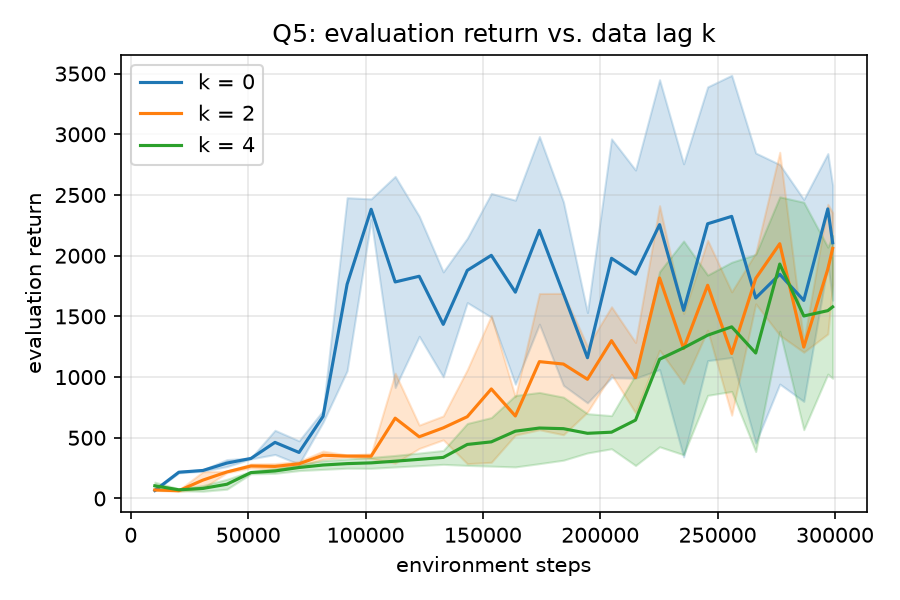
\includegraphics[width=0.62\linewidth]{q5_eval_return.png}
  \caption{Q5: evaluation return for $k\in\{0,2,4\}$ (clip loss).}
  \label{fig:q5ret}
\end{figure}

\begin{figure}[h]
  \centering
  \begin{subfigure}{0.49\linewidth}
    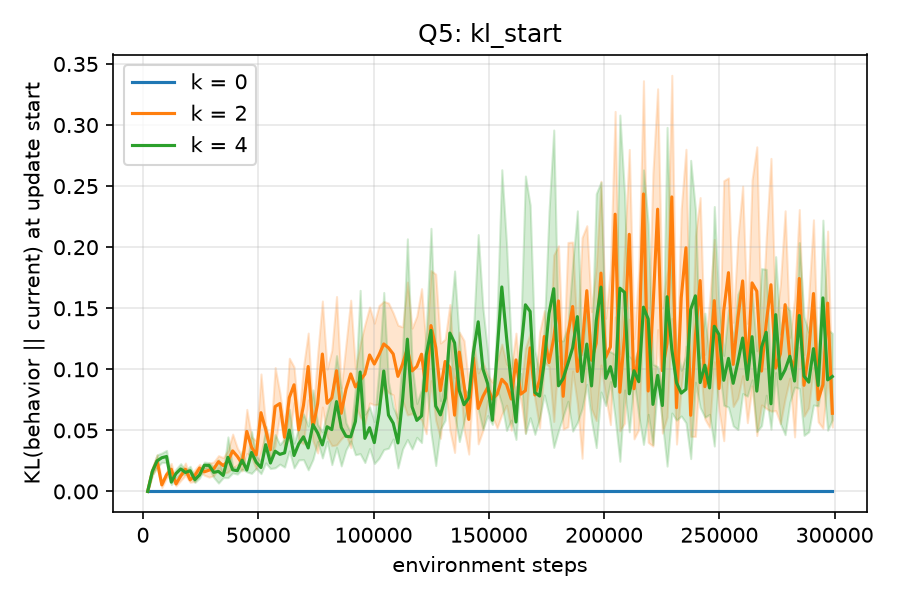
\includegraphics[width=\linewidth]{q5_kl_start.png}
    \caption{\code{kl\_start}}
  \end{subfigure}\hfill
  \begin{subfigure}{0.49\linewidth}
    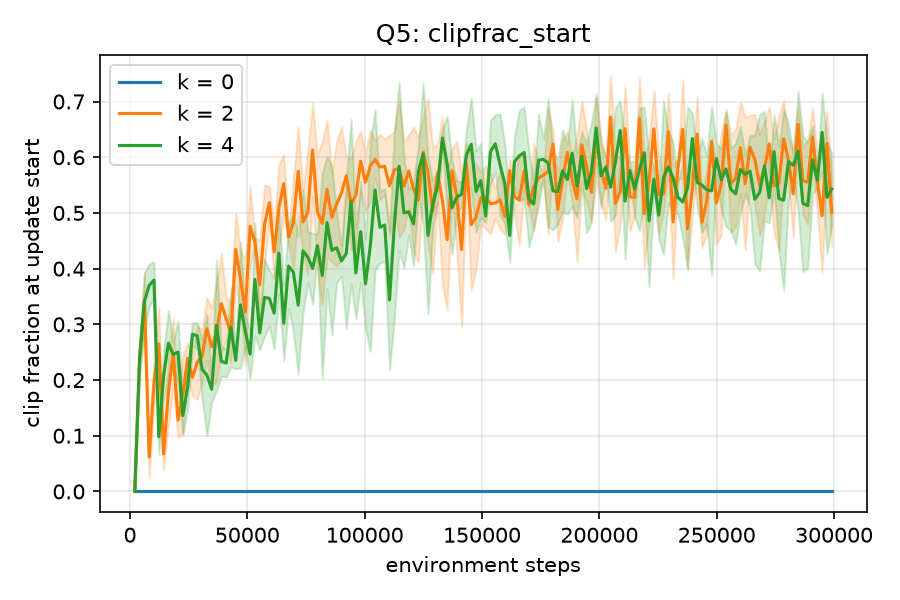
\includegraphics[width=\linewidth]{q5_clipfrac_start.png}
    \caption{\code{clipfrac\_start}}
  \end{subfigure}
  \caption{Q5: mismatch between the behavior policy and the current policy at the start of each update.}
  \label{fig:q5diag}
\end{figure}

\paragraph{Observations.}
\begin{itemize}[leftmargin=*]
  \item \textbf{Return} (Fig.~\ref{fig:q5ret}, Table~\ref{tab:summary}). Learning is clearly delayed by staleness.
        With $k=0$ all seeds pass a return of 1000 at about $1\times10^5$ steps. With $k=2$ this happens
        between $1.1\times10^5$ and $2.25\times10^5$, and with $k=4$ only after $2.1$--$2.6\times10^5$ steps. At $k=2$ the
        final return ($2060\pm294$) catches up with $k=0$ ($2106\pm473$), but the area under the curve is much
        smaller. At $k=4$ the final return is lower ($1578\pm588$) and the curve is still rising.

  \item \textbf{\code{kl\_start} and \code{clipfrac\_start}} (Fig.~\ref{fig:q5diag}). For $k=0$ both are exactly zero,
        a sanity check that the update starts on-policy ($r_\theta\equiv1$). For $k>0$ both grow during the
        first $\sim1.5\times10^5$ steps and then plateau at $\code{kl\_start}\approx0.1$--$0.13$ and
        $\code{clipfrac\_start}\approx0.55$--$0.6$. In the second half, the ratios at the start of the
        update are far from 1: the 5th/95th percentiles of $r_\theta$ are $0.39/1.83$ ($k=2$) and
        $0.41/1.81$ ($k=4$). So well over half the batch is outside $[1-\epsilon,1+\epsilon]$ before a
        single gradient step.

  \item \textbf{Unexpected result.} We expected $k=4$ to show a larger start-of-update mismatch than
        $k=2$, but the two plateaus overlap ($0.111$ vs.\ $0.126$, Table~\ref{tab:summary}). The
        explanation is in the end-of-update diagnostics: $\code{kl\_end}\approx0.013$ for every $k$,
        \emph{smaller} than \code{kl\_start}. So, measured against the stale behavior policy, each update
        moves the policy back towards $\pi_{\theta_{i-k}}$ (see (c)). Because every update re-anchors the
        policy to old data, the total drift between $\pi_{\theta_{i-k}}$ and $\pi_{\theta_i}$
        does not grow linearly with $k$; it saturates. In addition, $k=4$ learns
        more slowly, so its policy moves less per iteration, and keeps a larger entropy ($3.6$ vs.\ $3.4$). A wider
        Gaussian produces a smaller KL for the same mean shift.
\end{itemize}

\subsubsection*{(c) Analysis}

\paragraph{How stale can the data be?}
In this setup, performance already degrades at $k=2$: it reaches a return of 1000 roughly $1.2$--$2.4\times$ later than $k=0$, with larger seed
variance early on. The degradation becomes substantial at $k=4$, which ends lower and is still far from
converged at $3\times10^5$ steps. Only $k=0$ (truly on-policy) is free of the effect. PPO tolerates a small
lag in the sense that it does not diverge, which is clipping at work. But any lag that makes $r_\theta$
leave the trust region at the start of the update means more environment steps are needed to
reach the same return, i.e.\ lower sample efficiency.

\paragraph{Explanation using Q2.}
Even with exact advantages, the correctly reweighted gradient needs the full factor
$w_\theta(s)\,r_\theta(s,a)$, where $w_\theta(s)=d^{\pi_\theta}(s)/d^{\piold}(s)$. PPO uses only
$r_\theta$ and implicitly sets $w_\theta(s)\approx1$. The bound
$\|d^{\pi_\theta}-d^{\piold}\|_1\le\frac{2\gamma}{1-\gamma}\E_{s\sim d^{\piold}}[D_{TV}]$ says
this approximation is only justified while the two policies are close. With $\gamma=0.99$ the
factor in front is $2\gamma/(1-\gamma)=198$, and the left-hand side can never exceed 2. So the
bound only tells us something when the average $D_{TV}$ is below about $0.01$. With
\code{kl\_start}$\,\approx0.12$ and more than half of the ratios outside $[0.8,1.2]$, the
policies are far from that close, and the bound gives no guarantee that the state
distributions are similar. The data are therefore drawn from $d^{\pi_{\theta_{i-k}}}$, which may
differ substantially from $d^{\pi_{\theta_i}}$, and the gradient puts weight on states the
current policy no longer visits and too little on states it does visit. In addition, $\Ahat\approx A^{\pi_{\theta_{i-k}}}\neq A^{\pi_{\theta_i}}$ (Q3b), a
second error that also grows with the policy gap.

\paragraph{Explanation using Q4.}
$w_\theta$ cannot be computed because $d^{\pi}=(1-\gamma)(I-\gamma P_\pi^\top)^{-1}p_0$ depends
on the unknown transition kernel and, through the matrix inverse, on the policy at \emph{all} states.
Changing the policy at one state changes $P_\pi$ in that row, and the inverse spreads the change to every
state reachable from it. In Hopper, slightly different joint torques early in an episode
lead to different gaits, heights and fall times, so after $k$ iterations of learning, the states
visited by $\pi_{\theta_{i-k}}$ (e.g.\ falling after a short hop) are systematically different from those
of $\pi_{\theta_i}$ (longer hopping). The stale rollout's states are simply the wrong states to improve
the current policy on, and nothing in the loss corrects for this.

\paragraph{The clip fraction and the fraction of useful samples.}
For a sample with ratio $r$ and advantage $\Ahat$, the clipped objective (maximised by PPO) is
\begin{center}
  $\min\big(r\Ahat,\ \mathrm{clip}(r, 1-\epsilon, 1+\epsilon)\Ahat\big)$.
\end{center}
If $r$ is within $[1-\epsilon, 1+\epsilon]$, i.e.\ $|r-1|\le\epsilon$, both branches are equal and
the gradient is $\Ahat\nabla_\theta r$, which is non-zero whenever $\Ahat\neq0$. So every in-range
sample contributes. If $r$ is out of range ($|r-1|>\epsilon$), there are two cases:
\begin{itemize}[nosep]
  \item $r>1+\epsilon,\ \Ahat>0$ or $r<1-\epsilon,\ \Ahat<0$: the $\min$ selects the
        \emph{clipped} branch, which is constant in $\theta$, so the gradient is zero. The policy has
        already moved in the direction the advantage asks for.
  \item $r>1+\epsilon,\ \Ahat<0$ or $r<1-\epsilon,\ \Ahat>0$: the $\min$ selects the
        \emph{unclipped} branch $r\Ahat$, so the gradient $\Ahat\nabla_\theta r$ is non-zero. It pushes
        $r$ back towards 1, i.e.\ the current policy $\pi_{\theta_i}$ towards the stale policy
        $\pi_{\theta_{i-k}}$.
\end{itemize}
The indicator $\mathbf{1}[|r_i - 1| > \epsilon]$ marks sample $i\in\{1,\dots,N\}$ as out of range, so
$\code{clipfrac} = \frac{1}{N}\sum_i \mathbf{1}[|r_i - 1| > \epsilon]$ is the fraction of
out-of-range samples, and $1-\code{clipfrac}$ is the fraction of in-range samples, all of which
contribute a gradient. This is only a lower bound because out-of-range samples in the second case
above also contribute a non-zero gradient but are not counted. With stale data this case is
common, since $\Ahat$ was estimated without regard to the direction in which the policy has moved
over the last $k$ iterations. Also, \code{clipfrac\_start} is only a snapshot: during the 10 epochs
some samples enter and leave the clipping region.

Our results show why this matters. For $k\in\{2,4\}$, $1-\code{clipfrac\_start}\approx0.43$, so
fewer than half the samples are guaranteed to give a normal policy-gradient signal. Many of the
remaining non-zero gradients come from the second case above and pull the policy back towards the
stale behavior policy. This matches the drop from $\code{kl\_start}\approx0.12$ to
$\code{kl\_end}\approx0.013$ and from $\code{clipfrac}\approx0.57$ to $0.18$. Much of each update is
spent pulling the policy back into a trust region centred on an outdated policy, rather than
improving the current one. This explains the slower learning in Fig.~\ref{fig:q5ret}.

\paragraph{Why PPO discards its data after every iteration.}
Reusing a rollout after the policy has moved has three effects:
\begin{enumerate}
  \item The number of samples with an informative clipped gradient shrinks ($1-\code{clipfrac}$
        falls from 1 to $\approx0.43$).
  \item The trust region is centred on the wrong policy, so updates partly undo progress.
  \item The uncorrected state-distribution mismatch $w_\theta(s)$ and advantage mismatch
        $A^{\pi_\theta}\neq A^{\piold}$ grow with the policy gap and bias the gradient.
\end{enumerate}
Clipping keeps the procedure stable but cannot remove any of these effects. A fresh rollout costs
only 2048 environment steps, and it restores $r_\theta\equiv1$, $w_\theta\equiv1$ and
$A^{\pi_\theta}=A^{\piold}$ at the start of the update. Reusing older data instead buys nothing
(in our runs every $k$ collects the same number of steps) and adds the three effects above. So
PPO stays (almost) on-policy: it reuses each rollout only for the 10 epochs of one iteration,
where the policy is kept close by design.

%=====================================================================
\subsection*{Q6: Does the Importance Ratio Help with Stale Data?}

\subsubsection*{(a) Modification and equality of gradients}

\paragraph{Implementation} (\code{ppo.py}). \code{PPOAgent} takes \code{loss\_type}$\in\{$\code{naive},
\code{ratio}, \code{clip}$\}$, selected with \code{--loss} in \code{train.py}. With
\code{ratio = exp(newlogprob - b\_logprobs)} and the normalized advantages:
\begin{align*}
  \text{naive:} & \quad \code{pg\_loss} = -\Ehat[\log\pi_\theta(a\mid s)\,\Ahat],                                                           \\
  \text{ratio:} & \quad \code{pg\_loss} = -\Ehat[r_\theta(s,a)\,\Ahat],                                                                     \\
  \text{clip:}  & \quad \code{pg\_loss} = -\Ehat\big[\min\big(r_\theta\Ahat,\ \mathrm{clip}(r_\theta,1-\epsilon,1+\epsilon)\Ahat\big)\big].
\end{align*}
The value loss, gradient clipping, advantage normalization (once per rollout) and the stored behavior
log-probabilities are identical for all three.

\paragraph{Equal gradients at $r_\theta=1$.}
$\Ahat$ and $\log\piold(a\mid s)$ do not depend on $\theta$. Since
$r_\theta=\exp(\log\pi_\theta-\log\piold)$,
\[
  \nabla_\theta r_\theta(s,a) = r_\theta(s,a)\,\nabla_\theta\log\pi_\theta(a\mid s).
\]
\begin{itemize}[leftmargin=*]
  \item Naive: $\nabla_\theta L_{\text{naive}} = -\Ehat[\Ahat\,\nabla_\theta\log\pi_\theta]$.
  \item Ratio: $\nabla_\theta L_{\text{ratio}} = -\Ehat[\Ahat\,r_\theta\,\nabla_\theta\log\pi_\theta]$, which equals the naive
        gradient when $r_\theta=1$ for every sample.
  \item Clip: at $r_\theta=1$ we have $1-\epsilon<r_\theta<1+\epsilon$ (for $\epsilon>0$), so
        $\mathrm{clip}(r_\theta,1-\epsilon,1+\epsilon)=r_\theta$ in a neighbourhood of this point. Both arguments of
        the $\min$ coincide and equal $r_\theta\Ahat$, so the per-sample objective is locally $r_\theta\Ahat$
        and its gradient is $\Ahat\nabla_\theta r_\theta=\Ahat\,r_\theta\nabla_\theta\log\pi_\theta=\Ahat\nabla_\theta\log\pi_\theta$.
\end{itemize}
So all three losses have the gradient $-\Ehat[\Ahat\,\nabla_\theta\log\pi_\theta(a\mid s)]$, the
standard on-policy policy gradient. This is exactly the situation at the first mini-batch of an update with
$k=0$. The losses differ only once $r_\theta\neq1$, i.e.\ for stale data or after the first gradient step.

\subsubsection*{(b) Results}

\begin{figure}[h]
  \centering
  \begin{subfigure}{0.49\linewidth}
    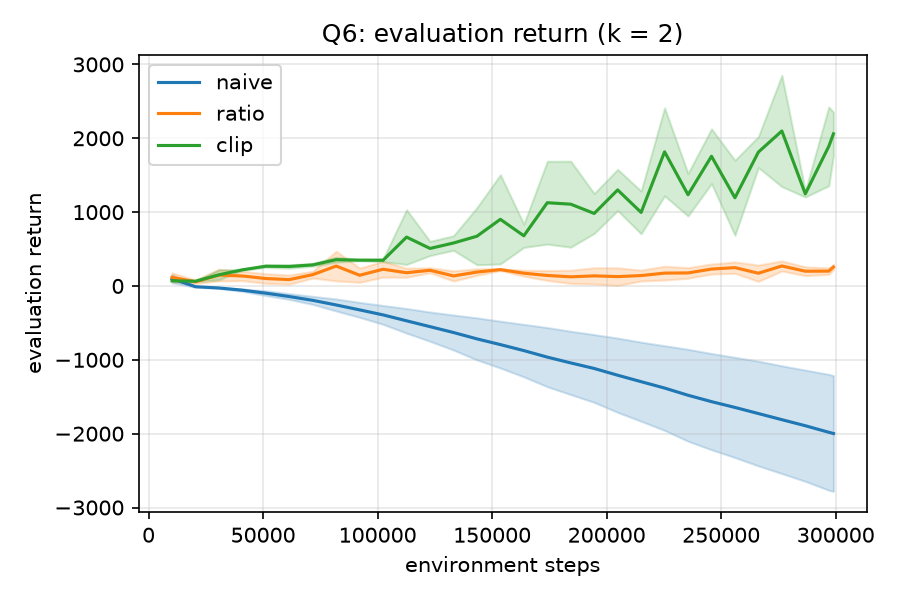
\includegraphics[width=\linewidth]{q6_eval_return.png}
    \caption{evaluation return}
  \end{subfigure}\hfill
  \begin{subfigure}{0.49\linewidth}
    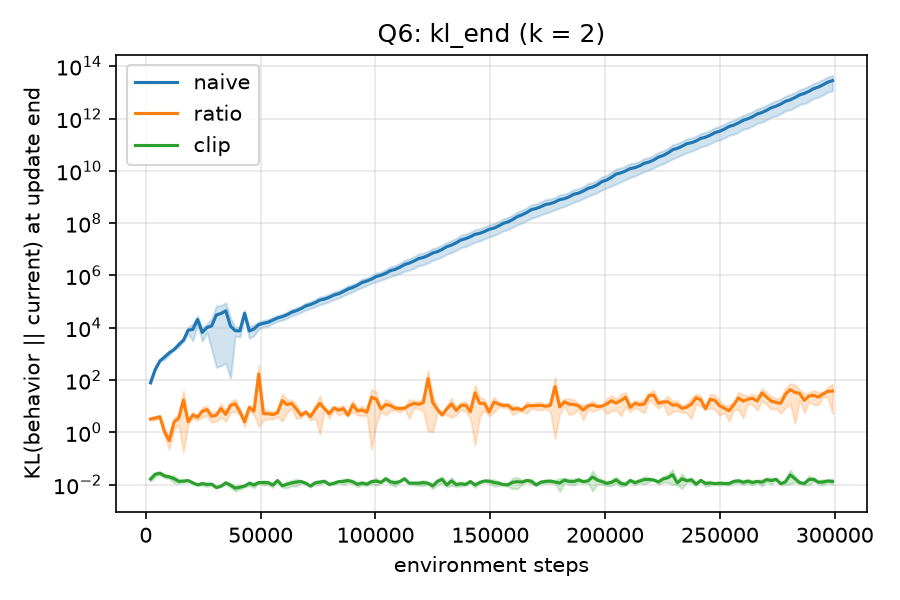
\includegraphics[width=\linewidth]{q6_kl_end.png}
    \caption{\code{kl\_end} (log scale)}
  \end{subfigure}
  \caption{Q6: the three surrogate losses with $k=2$. The clip curve is the $k=2$ run from Q5.}
  \label{fig:q6}
\end{figure}

\begin{itemize}[leftmargin=*]
  \item \textbf{clip} learns normally (final $2060\pm294$) with $\code{kl\_end}\approx0.01$--$0.02$ throughout.
  \item \textbf{ratio} makes almost no progress. The return stays at $100$--$400$ (final $256\pm36$), about the level
        of a policy that stands and falls. Its \code{kl\_end} is $\sim1$--$100$ (mean $16.6$ in the second half), three orders of magnitude
        above clip, and $97\%$ of samples end the update outside the trust region. The median ratio at the end of an
        update is $0.01$ and the entropy becomes negative ($4.2\to-2.2$ for seed 1), i.e.\ the policy collapses.
  \item \textbf{naive} is the worst. The return decreases monotonically from the first evaluation and reaches
        $-1998\pm784$. Its \code{kl\_end} is already $\approx 90$ after the first update and then grows
        \emph{exponentially} (a straight line on the log plot) to $\sim10^{13}$. The entropy falls to $\approx-17$
        ($-23$ for seed 1, i.e.\ $\log\sigma\approx-9$ per action dimension).
  \item \textbf{Numerical stability.} No run produced a non-finite loss or KL, so all 146 iterations
        are available for every configuration and no truncation was needed. The naive run is, however,
        numerically degenerate: its ratios underflow to $0$ for essentially all samples
        ($95$th percentile $\approx10^{-17}$) and its value loss is $\sim10^5$.
\end{itemize}

\subsubsection*{(c) Analysis}

\paragraph{Without the ratio (naive).}
The naive loss ignores where the data came from. It treats $(s,a)\sim\piold$ as if it were drawn from
$\pi_\theta$, so it lacks \emph{both} corrections of Q3(a): $w_\theta(s)$ and $r_\theta(s,a)$. Even in
expectation it is not the gradient of $J(\theta)$ once $\theta\neq\theta_{\mathrm{old}}$. More
damaging, it has no term that anchors $\theta$ near $\theta_{\mathrm{old}}$, and the objective it maximizes,
$\Ehat[\Ahat\log\pi_\theta]$, is \emph{unbounded above}. For a Gaussian policy,
\[
  \Ahat_i\log\pi_\theta(a_i\mid s_i) = -\Ahat_i\frac{\|a_i-\mu_\theta(s_i)\|^2_{\Sigma^{-1}}}{2}
  - \Ahat_i\sum_j\log\sigma_j + \text{const}.
\]
For a sample with $\Ahat_i<0$, this term grows without bound as $\mu_\theta(s_i)$ moves away
from $a_i$. Shrinking $\sigma$ multiplies that growth by $1/\sigma^2$. Positive-advantage samples bound their own term
by $0$ but cannot balance this. The $\log\sigma$ terms cancel on average because the advantages are normalized
to zero mean. Ten epochs of Adam on this objective therefore drive $\sigma\to0$
(entropy $\to-17$) and push the mean away from the actions that did badly, to arbitrarily large values. So the KL grows
geometrically, at a rate set by the learning rate, as observed. Huge action magnitudes explain the
\emph{negative} returns: Hopper's control cost $10^{-3}\|a\|^2$ is computed on the raw action, so it
dominates the healthy and forward rewards. The failure modes without the ratio are a biased gradient that is not
the policy gradient of any nearby policy, combined with an unbounded objective that leads to divergence and entropy
collapse. Note that the gradient is never weighted by how likely the sample is under the current
policy, so a sample the current policy would never generate still produces a full-size gradient.

\paragraph{With the ratio but without clipping (ratio).}
Weighting by $r_\theta$ restores the action-distribution correction. In expectation,
$\Ehat[r_\theta\nabla\log\pi_\theta\,\Ahat]$ is the Q3(b) estimator, which corrects $a\sim\piold$ to
$a\sim\pi_\theta$ but still assumes $w_\theta(s)\approx1$ and $A^{\pi_\theta}\approx A^{\piold}$.
This is why ratio does much better than naive (no divergence, positive return). But:
\begin{enumerate}[nosep,leftmargin=*]
  \item \textbf{Unbounded surrogate.} $r\Ahat$ grows without bound as $r\to\infty$ for $\Ahat>0$, and the gain is bounded by
        $0$ as $r\to0$ for $\Ahat<0$. Optimizing it for 10 epochs concentrates probability mass on a few
        positive-advantage actions. The policy narrows (negative entropy), most stored actions become improbable
        (median $r_{\text{end}}=0.01$), and a handful of samples with large $r$ dominate the batch.
  \item \textbf{High variance.} With $r$ spread over several orders of magnitude, the importance-weighted
        gradient has a very large variance. Its effective sample size is a small fraction of 2048, so the gradient is
        noise-dominated, which explains the stalled return.
  \item \textbf{Approximations break down.} Since $\code{kl}\sim10$, the policies are far apart. Then
        $w_\theta(s)\approx1$ and $A^{\pi_\theta}\approx A^{\piold}$ (Q2, Q3b) are badly violated: the surrogate
        $\Ehat[r\Ahat]$ is only a first-order local approximation of $J(\theta)-J(\theta_{\mathrm{old}})$, so maximizing it
        far from $\theta_{\mathrm{old}}$ no longer improves the true return.
\end{enumerate}
In short, the ratio fixes the bias in the action distribution, but without a constraint the optimizer
exploits the surrogate in a region where it is meaningless and the importance weights have huge variance.

\paragraph{How clipping helps.}
The clipped objective is flat in $r$ once $r$ leaves $[1-\epsilon,1+\epsilon]$ in the improving
direction. This removes the incentive to push any sample's ratio further, which bounds the effective
importance weights and the variance of the gradient. It keeps $\pi_\theta$ close to $\piold$, where
$w_\theta\approx1$ and $A^{\pi_\theta}\approx A^{\piold}$ are reasonable (the bound in Q2b). The pessimistic $\min$
also leaves a gradient on samples where the policy moved in the wrong direction, pulling them back.
Empirically, $\code{kl\_end}\approx0.013$ for every $k$, compared with $\sim17$ (ratio) and $\sim10^{12}$ (naive).

\paragraph{What clipping does not fix.}
\begin{itemize}[nosep,leftmargin=*]
  \item It does not correct the state distribution: $w_\theta(s)$ is still set to $1$ (Q2, Q4).
  \item It does not correct the advantages: $\Ahat$ still estimates $A^{\piold}$ (with an approximate critic), not $A^{\pi_\theta}$ (Q3b).
  \item It does not remove the mismatch already present in stale data. The trust region is centred on
        $\piold=\pi_{\theta_{i-k}}$, not on the current policy, so at the start of an update $57\%$ of samples are already
        clipped and part of the update is spent pulling the policy back towards an outdated policy (Q5c). This is why
        clip with $k>0$ is stable but slower than $k=0$.
  \item It does not enforce a hard trust region. Clipping only removes the gradient of individual
        samples; the policy can still move further through the shared network parameters, through other samples, or over
        many epochs. It gives no guarantee on $D_{TV}$ or KL. That clip stays at $\code{kl}\approx0.01$ is an empirical
        property of these hyperparameters (10 epochs, small learning rate, gradient clipping), not a guarantee.
\end{itemize}
Clipping therefore makes PPO \emph{robust} to mildly off-policy data, but it does not make PPO an off-policy
algorithm. The full correction $w_\theta(s)\,r_\theta(s,a)$ with $A^{\pi_\theta}$ is still missing, which is why PPO
collects fresh data every iteration.

\end{document}
